\chapter{Introduction\label{cha:chapter1}}

% https://books.google.de/books?id=2D0jBgAAQBAJ&pg=PA24&lpg=PA24&dq=%22die+ordnung+im+chaos+und+das+chaos+in+der+ordnung%22&source=bl&ots=rvYkaFGk-4&sig=IIxjTsPfpBmAEi8DBvmtHX0WE3Y&hl=en&sa=X&ved=0ahUKEwiM3ayxpvzUAhXKZFAKHc2mDV8Q6AEINjAD#v=onepage&q=%22die%20ordnung%20im%20chaos%20und%20das%20chaos%20in%20der%20ordnung%22&f=false

"Oder in the chaos and chaos in the order." This is how Osterhold describes one if the two essential directions of the chaos theory. Furthermore he claims, "processes, procedures or structures appearing very disordered only prove to be chaotic prior to they are analyzed further." This philosophical approach can be directly transfered to computer science, especially the field of information retrieval, data mining and data processing. 

\section{Motivation\label{sec:moti}}

% https://www.emc.com/leadership/digital-universe/2014iview/executive-summary.htm
% https://www.w3.org/TR/xmlschema-2/#boolean

The todays unbounded growth of information digitally available suggests a massive and chaotic collection of data. An in 2014 published report by EMC claims that the digitalized data grow by 100\% every two years and will reach 44 zettabytes (10\textsuperscript{21} bytes) by 2020 - as many stars as known in the universe. 
\\\\
Data in general, but also massive amounts of data, are only valuable if they are utilized appropriately. Gaining deeper insights is the point of transformation, visualization or calculation on data available. From a technical as well as an economical point of view a high degree of automation is required for maximizing the efficiency, especially when it comes to handling a high number of information entities. A large variety of software solutions are available and enable automated date processing for numerous domains. The solutions capture all levels of abstraction and reach from end user desktop applications, e.g. Microsoft Excel, to low level software frameworks, e.g. Pythons NumPy. Electronic data processing boils down to applied math and therefor relies on data of a deterministic structure. In computer science and mathematics there are well known specifications to transform and represent data in a computer understandable format. The canonical form, database normalization and schema definitions are some of them. They are primary beneficial for generalizing data representation on abstraction levels, namely storing data in table-based format or specifying the order of bytes on hardware level. A second evenly important aspect is the reduction of storage overhead when using predefined formats.
\\\\
Over the last years specifications being as old as the computers itself find less and less supporters and therefor compliance. Mainly to mention here are the database and application level. Developments according to Moore's law and constantly decreasing  costs of volatile memory are the enabler of that ongoing trend. Computational and memory power permit a by far more chaotic fashion of information storage. To perform analysis on data for reasonable time and resource costs in the past it was essential to hold data in a well defined schema, i.e. the structure of the information entity with meta information about attributes and types, and unique storage format. Modern data management solutions and databases loosened that strict demands. Schema-less and document orientated database management systems allow information entities with a deviating set of attributes to be stored. Data management and retrieval systems even allow documents of different storage format to be maintained. This trend develops in the favor of the users on application side. Overhead on schema definition, restrictions due to backward compatibility or synchronization of parties and stakeholders almost vanishes. The new development is very well received in technical development and opens new challenges in different research areas.
\\\\
The drawbacks of the a development have since been discovered by consumers of such chaotic data. Initially claimed, that more powerful hardware resources even out the bumpy road is only true if the the precision of the result must not meet the maximum. However, instances exist in which a best possible outcome on data analysis is indispensable. Exposure to end consumers, highly sensible analysis or unification of a brought number of data sources are case that tend to demand the latter requirements to be met. Not only the contemporary style of handling and storing information has its disadvantages but also data which already come in a well defined schema often do not fulfill the required granularity and purity of data for above mentioned use cases. In such applications a high amount of manual work for quality assurance has to be invested. Under the consideration of a rich landscape of different information entity formats data cleansing by hand, review of know-how owners or restructuration is done. This is only feasible on a low number of entities to be audited and becomes time and cost intense on big amounts of data.
\\\\
The motivation of this work contracts the potential optimization leeway in data pre-processing applications. 

\section{Objective and Problem statement\label{sec:objective}}

What kind of problem do you adress? Which issues do you try to solve? What solution do you propose? What is your goal?
'This thesis describes an approach to combining X and Y... The aim of this work is to...'

\section{Scope and Target\label{sec:scope}}

The target of this work is to present an overview of techniques, technologies and approaches available in different fields of computer science to tackle the stated problem. Furthermore, promising and adequate    

Here you should describe what you will do and also what you will not do. Explain a little more specific than in the objective section. 'I will implement X on the platforms Y and Z based on technology A and B.'

Conclude this subsection with an image describing 'the big picture'. How does your solution fit into a larger environment? You may also add another image with the overall structure of your component.

'Figure \ref{fig:intro} shows Component X as part of ...' 
\\
\begin{figure}[htb]
  \centering
  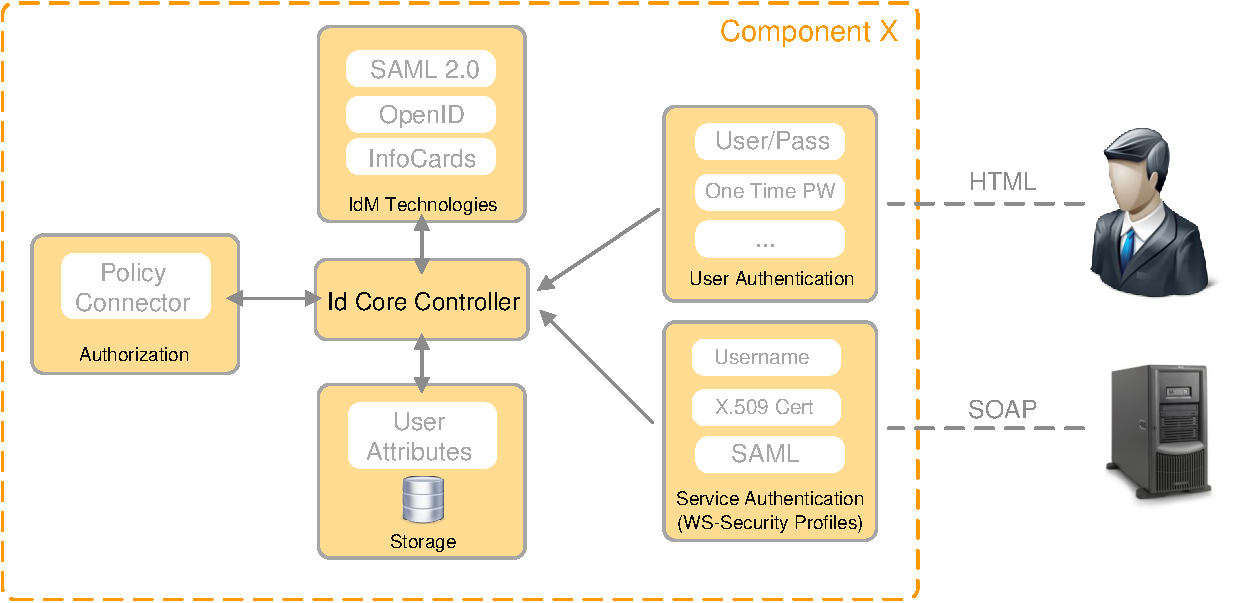
\includegraphics[width=9cm]{intro_example.pdf}\\
  \caption{Component X}\label{fig:intro}
\end{figure}

\section{Outline\label{sec:outline}}

The 'structure' or 'outline' section gives a brief introduction into the main chapters of your work. Write 2-5 lines about each chapter. Usually diploma thesis are separated into 6-8 main chapters. 
\\
\\
\noindent This example thesis is separated into 7 chapters.
\\
\\
\textbf{Chapter \ref{cha:chapter2}} is usually termed 'Related Work', 'State of the Art' or 'Fundamentals'. Here you will describe relevant technologies and standards related to your topic. What did other scientists propose regarding your topic? This chapter makes about 20-30 percent of the complete thesis.
\\
\\
\textbf{Chapter \ref{cha:chapter3}} analyzes the requirements for your component. This chapter will have 5-10 pages.
\\
\\
\textbf{Chapter \ref{cha:chapter4}} is usually termed 'Concept', 'Design' or 'Model'. Here you describe your approach, give a high-level description to the architectural structure and to the single components that your solution consists of. Use structured images and UML diagrams for explanation. This chapter will have a volume of 20-30 percent of your thesis.
\\
\\
\textbf{Chapter \ref{cha:chapter5}} describes the implementation part of your work. Don't explain every code detail but emphasize important aspects of your implementation. This chapter will have a volume of 15-20 percent of your thesis.
\\
\\
\textbf{Chapter \ref{cha:chapter6}} is usually termed 'Evaluation' or 'Validation'. How did you test it? In which environment? How does it scale? Measurements, tests, screenshots. This chapter will have a volume of 10-15 percent of your thesis.
\\
\\
\textbf{Chapter \ref{cha:chapter7}} summarizes the thesis, describes the problems that occurred and gives an outlook about future work. Should have about 4-6 pages.